\section{The bias-variance relationship}\label{sec:bv}

Understanding over and under-fitting is very important to understanding the challenges faced when doing machine learning. As it turns out those concepts are fundamentally tied to the out-of-sample error, $E_{out}$, for which the mean squared error (MSE) cost function can be decomposed in three contributions\footnote{We show this derivation in appendix \ref{appendix:bias_variance}}, namely

\begin{align}\label{eq:bv_decomp}
E_{out} = \langle C(S, f(\boldsymbol{x}; \theta_{S_t}))\rangle_{S,\, \epsilon} = \text{Bias}^2 + \text{Variance} + \text{Noise}.
\end{align}

\noindent This expectation is rather compact and so before we move on to explaining the bias and variance start by elaborating on $S$ and $\epsilon$. Recall from equation \ref{eq:target} that we decompose the target values as a contribution from a true function $\hat{f}$, and an error term $\epsilon$

\begin{equation}
\hat{y}_i = \hat{f}(\boldsymbol{x}_i) + \epsilon.
\end{equation}

\noindent In this section, we assume that the noise is distributed as $\epsilon \sim \mathcal{N}(0, \sigma^2)$.

The expectation in equation \ref{eq:bv_decomp} is taken over a model with optimized parameters $\theta_{S_t}$, whose value are a function of the selected data used in the optimization, $S_t = \{(\hat{y}_i, \boldsymbol{x}_i)\}$. We can then view our model, $f(\boldsymbol{x}; \theta_{S_t})$, as a stochastic functional which varies over the selected data used for training. The expectation over $S$ is then an expectation over the set of different choices of training data.

With the derived quantities from appendix \ref{appendix:bias_variance}, and equation \ref{eq:target}, we can then define the bias as

\begin{equation}\label{eq:bias}
\text{Bias}^2 = \sum_i (\boldsymbol{\hat{y}}_i - \langle f(\boldsymbol{x}_i; \theta_{S_t})\rangle_S)^2.
\end{equation}

\noindent The bias term is analogous to the squared error cost and gives and estimate to the degree of under-fitting the model is susceptible to. Building on this we have the variance term 

\begin{equation}\label{eq:variance}
\text{Variance} = \sum_i \langle (f(\boldsymbol{x}_i; \theta_{S_t}) - \langle f(\boldsymbol{x}_i; \theta_{S_t}) \rangle_S)\rangle_S.
\end{equation}

\noindent For clarity we note that the summation is over the testing set elements. The variance term relates to the consistency in the testing region, and as such describes the degree of over-fitting the model is exhibiting.

\begin{figure}
\centering
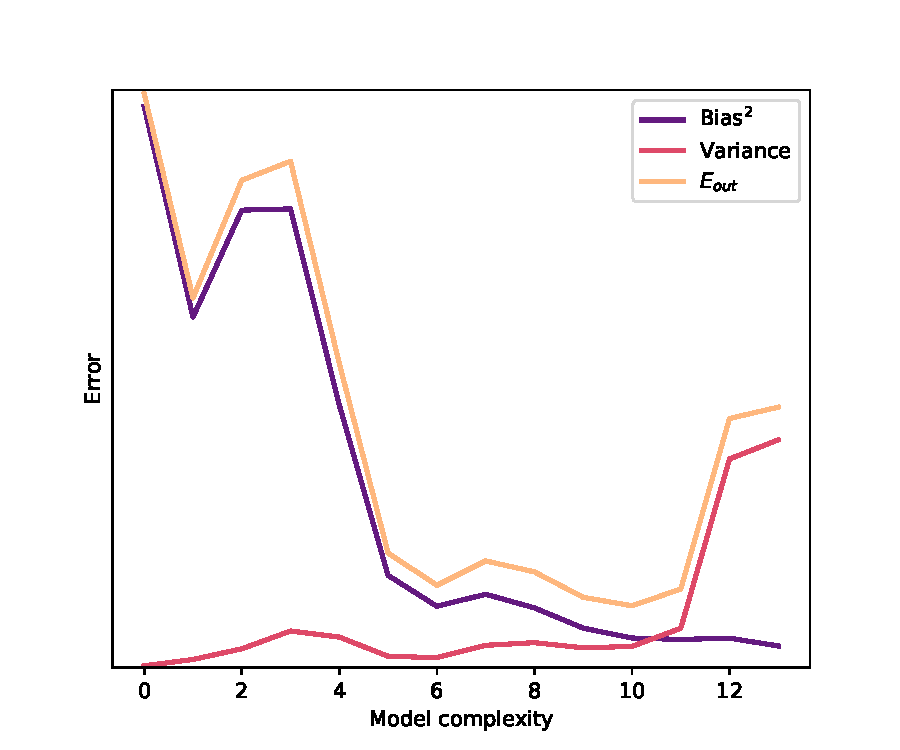
\includegraphics[width=0.55\textwidth, height=6.5cm]{../figures/bias_var_degree.pdf}
\caption[Bias-variance decomposition ]{Decomposition of the bias and variance from the overall test-set error $E_{out}$. A set of polynomials of varying degrees are fit to a known function using randomly selected training samples. The polynomial degree is denoted by the x-axis label. With the set of polynomials we evaluate the bias and variance terms shown in equation \ref{eq:bias} and \ref{eq:variance}. In the figure we observe the characteristic relationship where the out of sample error decreases steadily with complexity until the models start to over-fit as measured by the variance, and the $E_{out}$ increases as a consequence.}\label{fig:bv}
\end{figure}

The bias-variance relationship describes a fundamental challenge in most domains of machine learning; fitting a more complex model requires more data. This relationship has led to an explosion in the acquisition of vast amounts of data in the private sector. We illustrate the bias-variance relationship in figure \ref{fig:bv}, where polynomials of varying degrees are fit to a linear combination of exponential functions. We observe the characteristic tension between bias and variance wherein the out of sample error $E_{out}$ starts out decreasing with complexity but increases exponentially as a threshold is reached. Note also that we illustrate the concept of the irreducible error that for a model class, i.e. polynomials, there is an irreducible error term owing to the contribution from the noise. 

 In experimental nuclear physics, we often have an abundance of data. The challenge faced by researchers was centred around the lack of computing power. As such, it was the advent of optimized tools for machine learning that opened the avenue to explore complex models in the analysis of nuclear physics experiments. 